\documentclass{article}
\usepackage[utf8]{inputenc}
\usepackage{titling}
\usepackage{pgfgantt}
\usepackage{graphicx}
\usepackage{pdflscape}
\renewcommand{\refname}{Kaynakça}
\renewcommand{\figurename}{Resim}
\pretitle{
  \begin{center}
  \LARGE\bfseries
  
\includegraphics[width=0.2\textwidth]{ksbu.png} % Başlık önüne ekleyeceğiniz bir logo
  \vskip 1em
}
\title{Reinforcement Learning ile Yapay Zekaya Hayatta Kalmayı Öğretme}
\author{Hüseyin Buğra Taştan}
\date{25 Nisan 2024}

\begin{document}

    \maketitle
    \begin{center}
        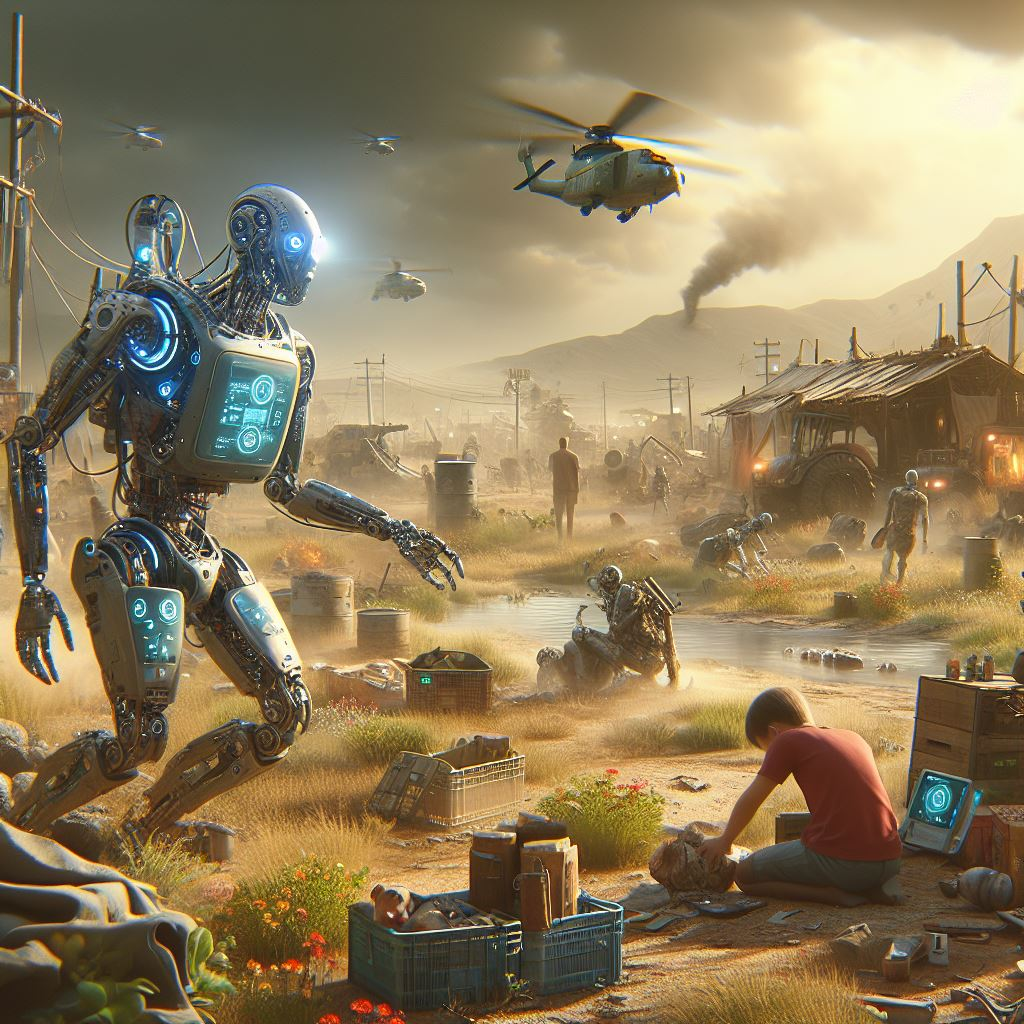
\includegraphics[width=0.4\textwidth]{forest.jpg} 
    \end{center}
    \vfill
    \rule{\textwidth}{0.5pt}
    \renewcommand{\abstractname}{Özet}
\begin{abstract}
\noindent "AI Learns To Survive" adlı proje, derin güçlendirme öğrenme (deep reinforcement learning) kullanarak yapay zeka ajanlarının hayatta kalma becerilerini öğrenmeye odaklanan bir araştırma veya uygulama projesidir. Projede amaç, yapay zeka ajanlarını belirli bir ortamda hayatta kalmaya yönlendirmek ve bu süreçte karşılaştıkları zorluklarla başa çıkabilmelerini sağlamaktır.
\end{abstract}
\rule{\textwidth}{0.5pt}
    \vfill

\newpage
\section{Giriş}
\rule{\textwidth}{0.5pt}
Günümüzde, yapay zeka teknolojisinin hızla gelişmesiyle birlikte, yapay zeka ajanlarının gerçek dünya ortamlarında başarılı bir şekilde işlev görmesi ve hatta hayatta kalabilmesi giderek daha büyük bir önem kazanıyor. "AI Learns To Survive" (Yapay Zeka Hayatta Kalmayı Öğreniyor) projesi, bu bağlamda derin güçlendirme öğrenme tekniklerini kullanarak yapay zeka ajanlarının hayatta kalma becerilerini geliştirmeye odaklanan heyecan verici bir araştırma ve uygulama girişimidir.Projemizin temel amacı, yapay zeka ajanlarını belirli bir ortamda hayatta kalmaya teşvik etmek ve bu süreçte karşılaşacakları çeşitli zorluklarla başa çıkabilmelerini sağlamaktır. Bu zorluklar, gerçek dünya senaryolarından esinlenmiş olabileceği gibi sanal ortamlarda da simüle edilebilir.Örneğin, bir robotun doğal afetler, engeller veya diğer tehlikelerle karşılaştığı bir ortamda hayatta kalabilme yeteneği üzerine odaklanabiliriz.Derin güçlendirme öğrenme algoritmaları, projemizin temelini oluşturur. Bu algoritmalar, yapay zeka ajanlarının ortama uyum sağlamak ve belirlenmiş hedefleri başarmak için optimal eylemleri öğrenmelerini sağlar. Öğrenme süreci genellikle bir ödül sistemiyle desteklenir; ajanlar belirli görevleri başarıyla tamamladıklarında veya belirli zorlukları aştıklarında ödüllendirilirler. Bu ödül sistemi, ajanların istenilen davranışları öğrenmelerini teşvik eder."Aİ Learns To Survive" projesi, yapay zeka alanında önemli bir boşluğu doldurmayı hedefliyor. Gerçek dünya uygulamalarında kullanılabilen yapay zeka ajanlarının, değişen ve bazen de tehlikeli ortamlarda başarılı bir şekilde işlev görebilmesi, teknolojinin ilerlemesinde kritik bir adımdır. Bu proje, bu hedefe ulaşmada bir adım daha atmaktadır.
  \newpage
  \section{Literatür Çalışması}
\rule{\textwidth}{0.5pt}
Bu makalede, derin pekiştirmeli öğrenme yöntemlerini kullanarak, yüksek boyutlu duyusal girdilerden (örneğin, görüntü veya konuşma gibi) doğrudan ajanları kontrol etmeyi öğrenmektir. Peşin başarılı pekiştirmeli öğrenme uygulamaları, bu tür alanlarda genellikle elle hazırlanmış özelliklerle birleştirilmiş doğrusal değer fonksiyonları veya politika temsillerine dayanmıştır\cite{mnih2013playing}.\\[15pt]

Bu makalede,derin pekiştirmeli öğrenme modellerini daha hızlı ve daha verimli bir şekilde eğitmek ve genişletmek için asenkron yöntemlerin etkin bir şekilde kullanılmasıdır. Bu sayede, daha karmaşık ve gerçekçi problemler üzerinde daha iyi performans gösteren yapay zeka sistemleri geliştirmek mümkün olabilir\cite{mnih2016asynchronous}.\\[15pt]

Bu projede, derin sinir ağları ve ağaç araması gibi ileri öğrenme tekniklerinin kullanılmasıyla, Go oyununu oynamak için daha etkili bir yaklaşım geliştirilmiştir. Derin sinir ağları, oyun tahtasındaki durumu analiz etmek ve olası hamleleri tahmin etmek için kullanılırken, ağaç araması algoritması, bu tahminleri daha ileri seviyeye taşımak ve olası hamlelerin sonuçlarını değerlendirmek için kullanılır\cite{silver2016mastering}.\\[15pt]

Bu proje, derin takviyeli öğrenme tekniklerini kullanarak genel video oyunları için yapay zeka geliştirmeyi amaçlamaktadır. Derin takviyeli öğrenme, yapay zeka ajanlarının belirli bir görevi gerçekleştirmek için çevreleriyle etkileşimde bulunarak deneyimlerinden öğrenmelerini sağlayan bir makine öğrenimi yaklaşımıdır.\cite{torrado2018deep}


\newpage


\clearpage


\section{ML Agents Nedir?}
ML Agents, Unity'nin yapay zeka ve makine öğrenimi modellerini eğitmek için geliştirilmiş bir araç setidir. Bu araç seti, Unity oyun motorunda oyun nesnelerini kontrol etmek için kullanılan yapay zeka algoritmalarını ve modellerini eğitmek için bir dizi araç ve kütüphane sunar. ML Agents, karmaşık oyun senaryolarında yapay zeka davranışlarını modellendirme ve eğitme sürecini kolaylaştırır.

\subsection{ML Agents Kullanımı}
ML Agents kullanarak yapay zeka modelleri eğitmek ve entegre etmek oldukça basittir. İşte temel adımlar:

\subsubsection{Çevrenin Tanımlanması}
İlk adım, yapay zeka modelini eğitmek için bir çevre tanımlamaktır. Bu çevre, oyun sahnesindeki nesneleri, hedefleri ve etkileşimleri içerir.

\subsubsection{Eğitim Verilerinin Toplanması}
Sonraki adım, çevrede yapay zeka modelini eğitmek için kullanılacak verilerin toplanmasıdır. Bu genellikle insan ya da önceden belirlenmiş stratejilerle oluşturulmuş verileri içerir.

\subsubsection{Yapay Zeka Modelinin Eğitimi}
Toplanan veriler kullanılarak yapay zeka modeli eğitilir. ML Agents, çeşitli makine öğrenimi tekniklerini destekler ve eğitim sürecini kolaylaştırır.

\subsubsection{Yapay Zeka'nın Entegrasyonu}
Eğitilen yapay zeka modeli, Unity oyun motoruna entegre edilir ve gerçek zamanlı olarak oyun sahnesinde kullanılır.
\clearpage
\section{Kurulum Aşamaları}
\begin{enumerate}
    \item Anaconda Kurulumu
    \item Unity Kurulumu
    \item ML-Agents Kurulumu
    \item Sanal Orrtam Oluşumu
    \item Gerekli Eklenti Kurulumları
    \item Eğitimin Başlatılması
\end{enumerate}
 \section{Proje Taslağı}
 Hayatta kalma oyunları genellikle oyuncuların doğal kaynakları toplamalarını, inşa etmelerini ve düşmanlardan kaçınmalarını veya onlarla savaşmalarını gerektirir. Yapay zeka, bu tür oyunlarda oyuncuların karşılaşabileceği düşman davranışlarını, kaynak toplama stratejilerini ve oyun dünyasıyla etkileşimlerini simüle etmek için kullanılabilir.
\begin{figure}[h]
    \centering
    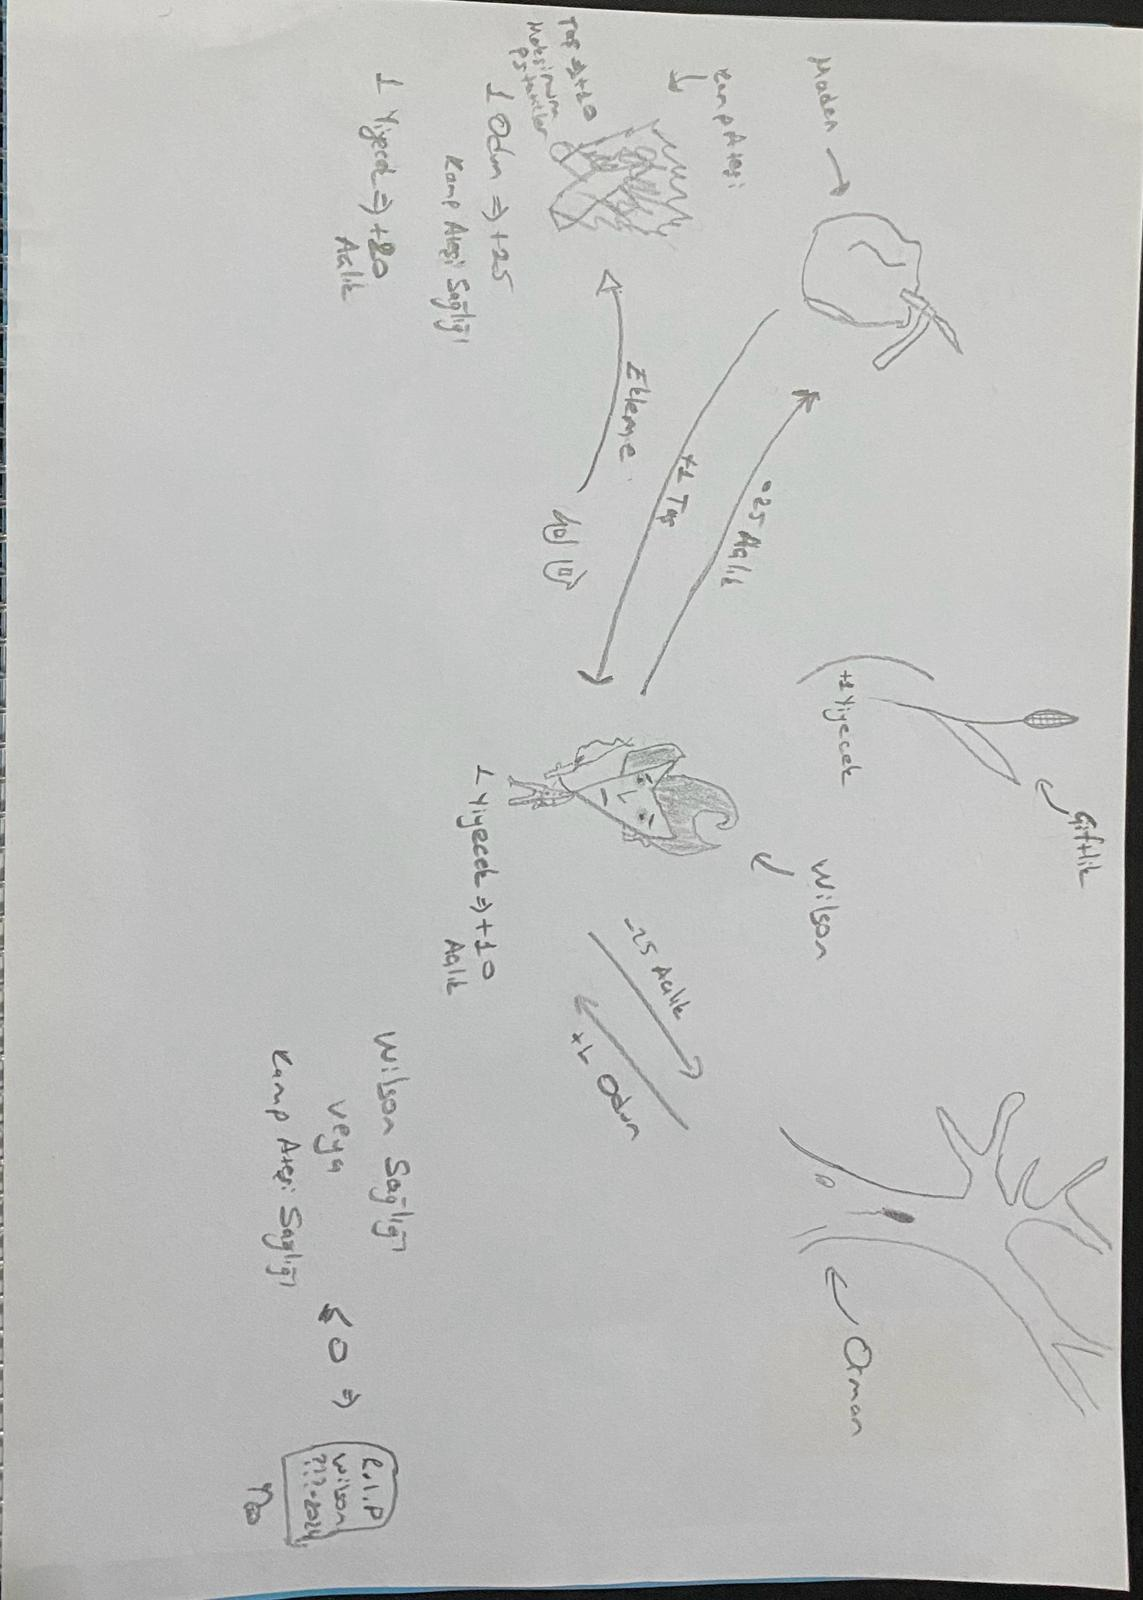
\includegraphics[angle=90,width=0.9\textwidth]{taslak.jpeg}
    \caption{Proje Taslağı}
    \label{fig:resim7}
\end{figure}
\clearpage
\section{Ortam Hazırlama Adımları}

\subsection{Temel Oyun Dünyası Oluşturma}

\begin{itemize}
\item \textbf{Proje Oluşturma:} Unity'de yeni bir proje oluşturun ve gerekli ayarları yapın.
\item \textbf{Sahne Oluşturma:} Sahneye bir arazi veya ortam ekleyin. Bu, oyunun geçeceği dünyayı temsil eder. Toprak, ağaçlar, kayalar gibi doğal unsurları içerebilir.
\item \textbf{Işıklandırma:} Işıklandırmayı ayarlayın. Gündüz ve gece döngüsü gibi dinamik ışıklandırma efektleri eklemek, oyun dünyasını daha gerçekçi hale getirebilir.
\item \textbf{Detaylar ve Atmosfer:} Ortama detaylar ekleyin; bitkiler, taşlar, su vb. Bunlar oyunun atmosferini zenginleştirecek ve oyuncuların etkileşimini artıracaktır.
\end{itemize}

\begin{figure}[h]
    \centering
    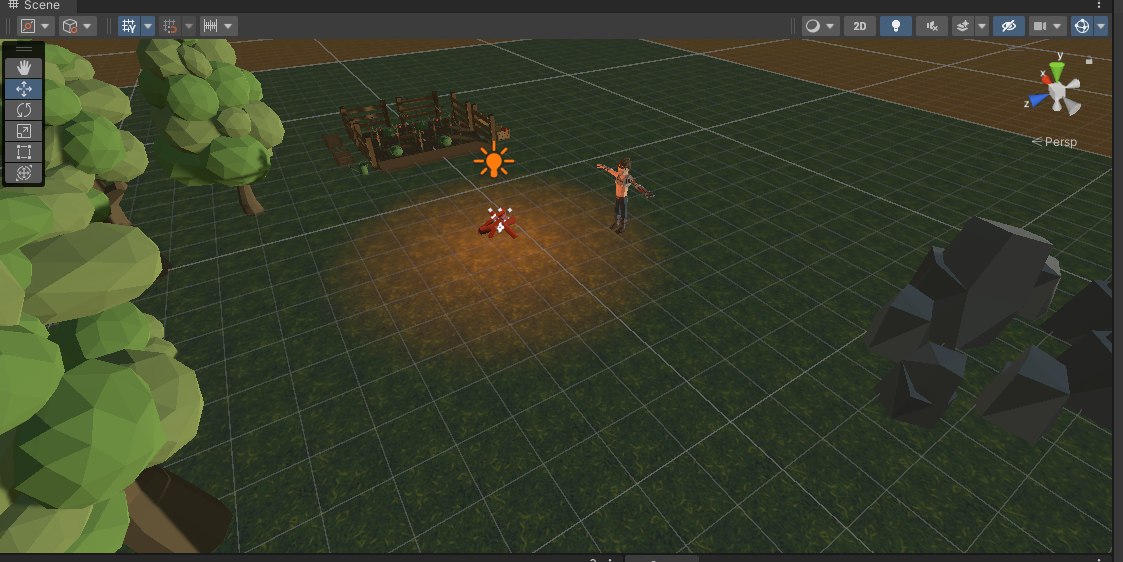
\includegraphics[width=0.9\textwidth]{unityortam.PNG}
    \caption{Ortam Oluşturma}
    \label{fig:resim8}
\end{figure}

\subsection{Yapay Zeka İçin Temel Unsurlar}
\begin{itemize}
\item \textbf{Düşman Karakterler:} Düşman karakterlerinizi tasarlayın ve oluşturun. Bu karakterler, oyuncuya karşı saldırabilir veya onlardan kaçabilir.
\item \textbf{Davranış Kodlaması:} Düşmanların hareket ve davranışlarını belirleyen temel kodları yazın veya hazır yapay zeka çözümlerini kullanın. Örneğin, düşmanların oyuncuyu takip etmesi veya belirli bir alanı savunması gerekebilir.
\item \textbf{Düşman AI Entegrasyonu:} Oyun içinde düşman yapay zekasını etkinleştirecek ve onların oyuncularla etkileşimini sağlayacak kodları entegre edin.
\end{itemize}

\subsection{Kaynak Toplama ve İnşa Etme Sistemleri}

\begin{itemize}
\item \textbf{Kaynakları Tanımlama:} Oyuncunun kaynakları toplayabileceği ve bunları kullanarak yapılar inşa edebileceği bir sistem oluşturun. Bu kaynaklar odun, taş, besin gibi şeyleri içerebilir.
\item \textbf{Yapıları Tanımlama:} Oyuncunun inşa edebileceği yapıları belirleyin. Bu yapılar barınaklar, savunma kuleleri, üretim tesisleri vb. olabilir.
\item \textbf{İnşa ve Üretim Mekanikleri:} Oyuncunun kaynaklarını kullanarak yapılar inşa etmesini ve bu yapılar aracılığıyla kaynakları işlemesini sağlayacak mekanikleri tasarlayın ve kodlayın.
\end{itemize}

\begin{figure}[h]
    \centering
    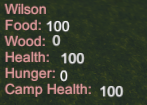
\includegraphics[width=0.9\textwidth]{kaynaklar.PNG}
    \caption{Kaynak Belirleme}
    \label{fig:resim9}
\end{figure}

\subsection{Yapay Zeka ile Etkileşimler}

\begin{itemize}
\item \textbf{Düşman Etkileşimleri:} Yapay zekanın kaynakları toplaması ve inşa etmesi için gerekli kodları yazın veya entegre edin. Ayrıca, düşmanların oyuncunun inşa ettiği yapıları hedef alması veya onları yok etmeye çalışması için gerekli kodları ekleyin.
\item \textbf{Oyuncu-Yapı Etkileşimleri:} Oyuncunun inşa ettiği yapılarla yapay zeka arasında etkileşimleri sağlayın. Örneğin, düşmanların oyuncunun inşa ettiği yapıları hedef alması veya bu yapıları savunması gerekebilir.
\end{itemize}

\section{Trigger Kullanımı}

Trigger'lar, bir nesnenin içine giren diğer bir nesne tarafından algılanan alanlardır. Bir nesne bir Trigger alanına girdiğinde, bu olay bir tetikleyici (trigger) olarak adlandırılır ve belirli bir işlevi başlatır. Örneğin, bir oyuncunun bir tarlaya girdiğinde bir tetikleyici tetiklenerek hasat yapabilir.

\begin{figure}[h]
    \centering
    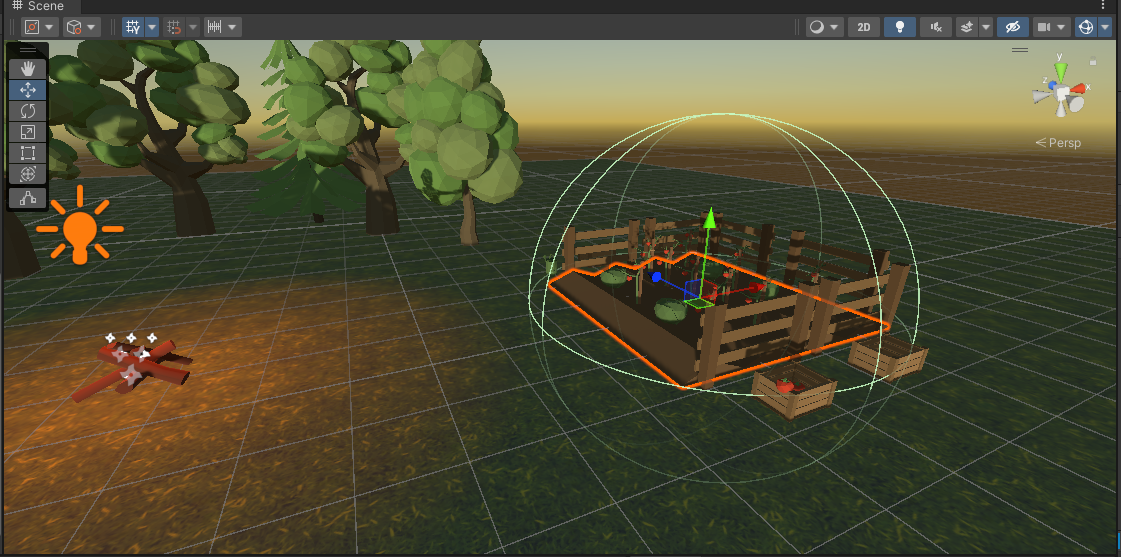
\includegraphics[width=0.9\textwidth]{collider.PNG}
    \caption{Trigger ve Collider Bileşeni}
    \label{fig:resim10}
\end{figure}

\subsection{Trigger'ı Etkinleştirme}

Unity'de bir nesnenin bir Trigger olarak işlev görmesi için, bir Collider bileşenine sahip olması ve "Is Trigger" özelliğinin etkinleştirilmiş olması gerekir.

\begin{figure}[h]
    \centering
    \includegraphics[width=0.9\textwidth]{triggeretkınlesme.PNG}
    \caption{Trigger Etkinleştirme}
    \label{fig:resim11}
\end{figure}
\clearpage
\subsection{Trigger Olayları}

Bir Trigger ile ilişkili olaylar genellikle OnTriggerStay, OnTriggerEnter ve OnTriggerExit fonksiyonlarıyla ele alınır. OnTriggerEnter, bir nesne Trigger alanına girdiğinde tetiklenir. OnTriggerStay, bir nesne Trigger alanında kaldığı sürece devam eder. Son olarak, OnTriggerExit, bir nesne Trigger alanından çıktığında tetiklenir.

\section{Collider Kullanımı}

Collider, nesnelerin fiziksel çarpışmalarını algılamak için kullanılır. İki nesne çarpıştığında, Collider'lar bu çarpışmayı algılar ve Unity'nin fizik motoruna bilgi gönderir, böylece nesneler arasındaki etkileşim gerçekleşir.

\subsection{Collider Türleri}

Unity'de farklı Collider türleri vardır, bunlar arasında BoxCollider, SphereCollider, CapsuleCollider, ve MeshCollider bulunur. Her biri farklı şekil ve formlara sahiptir ve nesnelerin çarpışma algılama şekillerini etkiler.
\subsection{Fiziksel Özellikler}

Collider'lar, nesnelerin fiziksel özelliklerini belirlemek için kullanılabilir. Örneğin, bir nesnenin ağırlığını, sürtünmesini ve elastikiyetini ayarlamak için Collider bileşeninin özellikleri kullanılabilir.

\begin{figure}[h]
    \centering
    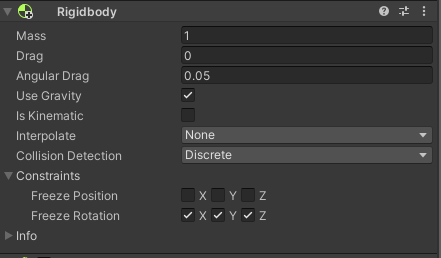
\includegraphics[width=0.9\textwidth]{rigidbody.PNG}
    \caption{Rigidbody}
    \label{fig:resim12}
\end{figure}
\clearpage
\section{Örnek Kod Parçası}

\begin{verbatim}
using UnityEngine;

public class yemek_hasat : MonoBehaviour
{
    
    private void OnTriggerEnter(Collider other)
    {
        Envanter.foodCount += 1;
        
    }
}
\end{verbatim}

\begin{verbatim}
using UnityEngine;
using TMPro;

public class Envanter : MonoBehaviour
{ 
    public static int foodCount = 0;
    
    [SerializeField] private TextMeshProUGUI foodText;

    // Güncelleme kare başına bir kez çağrılır
    void Update()
    {
        foodText.text = foodCount.ToString();

    }
}
\end{verbatim}

Yukarıdaki örnek, çiftliğin bir oyuncu tarafından hasat edilmesini sağlamak için bir Trigger kullanır. OnTriggerEnter fonksiyonu, oyuncu bir Trigger alanına girdiğinde tetiklenir ve foodCounta 1 ekler.
\clearpage

\section{Pekiştirmeli Öğrenme Algoritması}
\begin{figure}[h]
    \centering
    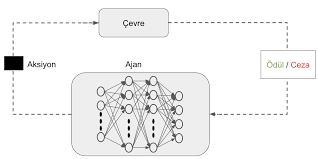
\includegraphics[width=0.8\textwidth]{ajantablosu.png}
    \caption{Makine Öğrenimi \cite{mnih013playing}} 
    \label{fig:resim13}
\end{figure}
\begin{enumerate}
    \item \textbf{Gözlemleme:} Model, çevresindeki ortamı gözler ve bu ortam hakkında bilgi toplar. Örneğin, bir video oyunundaki bir karakter, oyunun dünyasını ve karakterin durumunu gözlemleyebilir.
    \item \textbf{Karar Verme:} Model, mevcut gözlemlerine dayanarak bir eylem seçer. Bu eylem, belirli bir hedefe ulaşmak için tasarlanmıştır. Örneğin, bir video oyun karakteri, bir düşmanla savaşmak veya bir engeli aşmak için bir eylem seçebilir.
    \item \textbf{Eylemi Uygulama:} Model seçilen eylemi gerçekleştirir ve çevrede bir değişiklik oluşturur. Örneğin, bir video oyununda karakter hareket eder veya bir silah ateş eder.
    \item \textbf{Geri Bildirim Alınması:} Model, geri bildirim alır. Bu geri bildirim, seçilen eylemin ne kadar başarılı veya başarısız olduğunu belirtir. Örneğin, karakterin canını azaltan bir düşman saldırısı veya bir hedefi vurma başarısı olabilir.
    \item \textbf{Ödül veya Cezalandırma:} Model, aldığı geri bildirime göre bir ödül veya ceza alır. Eylem başarılıysa, genellikle bir ödül alır; başarısızsa bir ceza alır. Örneğin, düşmanı yenmek başarı olarak kabul edilirken, bir engelde takılıp kalmak cezalandırılır.
    \item \textbf{Öğrenme:}Model, aldığı geri bildirime dayanarak öğrenir. Başarılı eylemleri teşvik eden davranışları öğrenirken, başarısız eylemlerden kaçınmayı öğrenir.
    \item \textbf {Yeniden Gözlemleme ve Yeniden Karar Verme:} Model, güncel gözlemlerine dayanarak yeni bir eylem seçer ve süreç tekrarlanır.
\end{enumerate}

    
\section{ML-Agents İçin Gelişmiş Kavramlar}
    Unity ML-Agents'in temel kavramlarına hakim olduktan sonra, gelişmiş teknikler ve kavramlarla daha derinlemesine bir anlayış geliştirebiliriz. Bu bölümde, ML-Agents için önemli olan birkaç gelişmiş kavramı ele alacağız:

    \subsection{Reward Shaping}
        Reward Shaping, ajanın davranışlarını yönlendirmek ve hızlandırmak için ödüllendirme işlemine ek olarak kullanılan bir tekniktir. Bu teknik, ajanın istenen davranışları daha hızlı öğrenmesini sağlayabilir, ancak dikkatlice uygulanmalıdır çünkü yanlış bir şekilde kullanıldığında ajanın performansını olumsuz etkileyebilir.

        \begin{figure}[h]
    \centering
    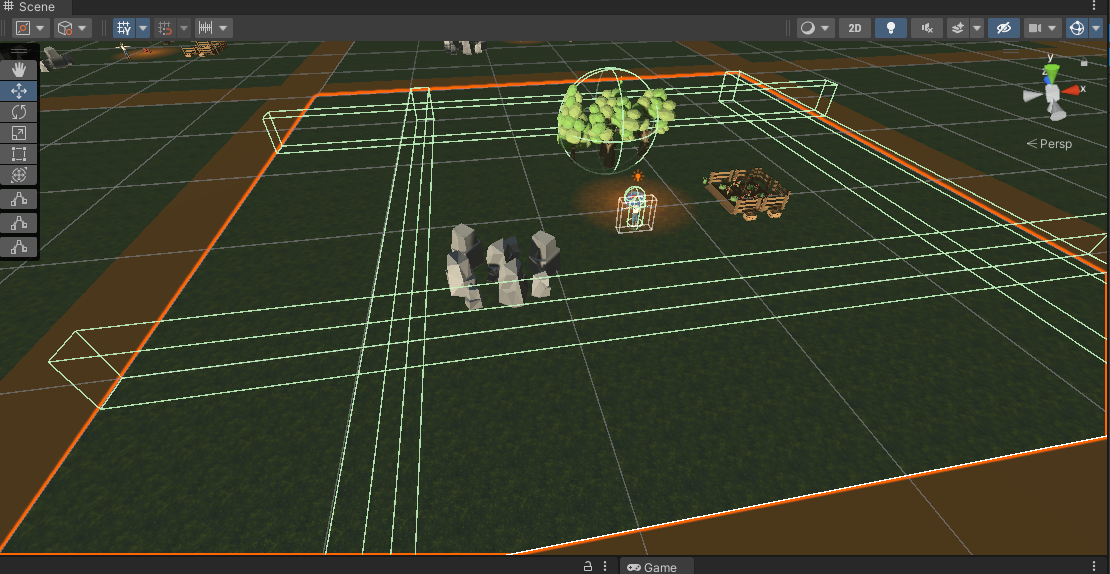
\includegraphics[width=0.7\textwidth]{odulceza.PNG}
    \caption{Ödül Ceza Sistemi}
    \label{fig:resim14}
    \end{figure}
    

    \subsection{Curriculum Learning}
        Curriculum Learning, ajanın öğrenme sürecini daha etkili hale getirmek için kullanılan bir öğrenme stratejisidir. Bu strateji, ajanın daha basit görevlerle başlamasını ve daha sonra giderek zorlaşan görevlere geçiş yapmasını sağlar. Bu, ajanın daha hızlı ve daha kararlı bir şekilde öğrenmesini sağlayabilir.
        \vspace{0,15cm}
        \footnotesize
        \begin{verbatim}
        private void OnTriggerEnter(Collider other)
        {
            if(other.gameObject.tag=="odun")
            {
                AddReward(10f);
                EndEpisode();
            }
            if(other.gameObject.tag=="wall")
            {
                AddReward(-5f);
                EndEpisode();
            }
        }
\end{verbatim}
        \clearpage

    \subsection{Proximal Policy Optimization (PPO)}
        PPO, ML-Agents'te sıkça kullanılan bir eğitim algoritmasıdır. Policy gradient metotlarının bir türü olan PPO, stabil ve hızlı bir şekilde ajanları eğitmek için tasarlanmıştır. Ayrıca, genellikle büyük ölçekli eğitim setleri üzerinde etkili bir şekilde çalışır.
        \begin{figure}[h]
    \centering
    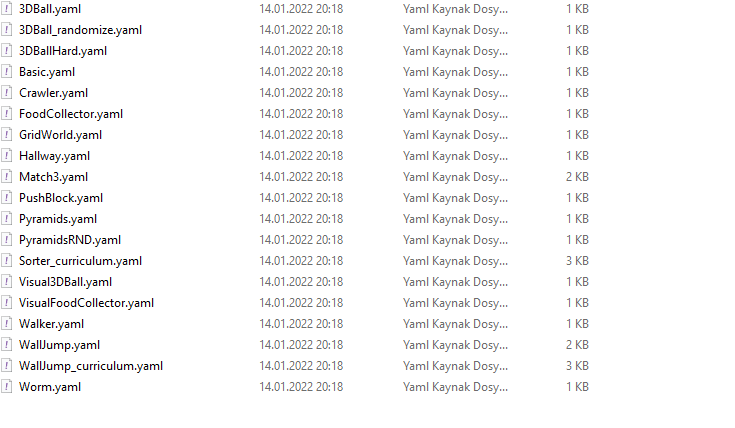
\includegraphics[width=0.9\textwidth]{yaml.PNG}
    \caption{PPO Örnek Dosyalar}
    \label{fig:resim15}
\end{figure}


\section{Gelişmiş Ortam Tasarımı}
    Gelişmiş bir ML-Agents ortamı tasarlarken dikkate alınması gereken birkaç önemli faktör bulunmaktadır. Bu bölümde, ML-Agents ile gelişmiş ortamların tasarımı ve yönetimi üzerine bazı ipuçlarını ele alacağız:

    \subsection{Kompleks Ortamların Oluşturulması}
        ML-Agents ile kompleks ve etkileşimli ortamlar oluşturmak için Unity'nin özelliklerinden yararlanabiliriz. Bu, ajanların gerçek dünya senaryolarına daha yakın bir şekilde eğitilmesini sağlayabilir.

    \subsection{Çoklu Ajan Ortamları}
        ML-Agents, birden fazla ajanı aynı ortamda eğitmeyi ve simüle etmeyi destekler. Bu, işbirliği ve rekabet temelli senaryolar için idealdir. Çoklu ajan ortamları tasarlarken dikkat edilmesi gereken özel durumlar bulunmaktadır.
        \begin{figure}[h]
    \centering
    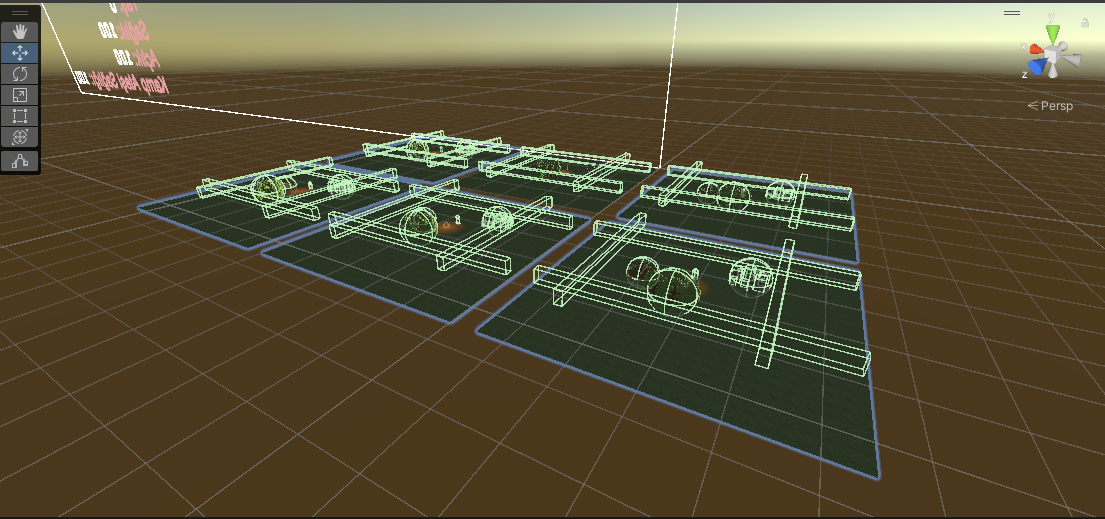
\includegraphics[width=0.9\textwidth]{genelgorunum.PNG}
    \caption{Çoklu Eğitim Örneği}
    \label{fig:resim16}
\end{figure}

    
\section{Ajanların Gelişmiş Eğitimi}
    Ajanların gelişmiş eğitimi, ML-Agents kullanıcılarının sık sık karşılaştığı bir konudur. Bu bölümde, ajanların daha hızlı, daha stabil ve daha verimli bir şekilde eğitilmesini sağlamak için kullanılan bazı gelişmiş eğitim tekniklerini ele alacağız:

    \subsection{Eğitim Hiperparametrelerinin Ayarlanması}
        ML-Agents eğitim sürecinde birçok hiperparametre vardır ve bu parametrelerin doğru bir şekilde ayarlanması önemlidir. Örneğin, öğrenme hızı, eğitim devri sayısı, ödül şekillendirme faktörleri gibi parametrelerin dikkatlice ayarlanması gerekebilir.

    \subsection{Eğitim Verimliliğini Artırmak İçin Teknikler}
        Ajanların eğitim verimliliğini artırmak için birçok teknik mevcuttur. Bunlar arasında deneyim tekrarı, örnek çeşitliliği sağlama, eğitim verilerinin dengelemesi gibi teknikler bulunabilir. Bu teknikler, ajanların daha hızlı ve daha stabil bir şekilde öğrenmelerini sağlayabilir.

    \subsection{Hızlandırılmış Eğitim için Paralel Eğitim}
        ML-Agents, paralel eğitim modunu destekler. Bu, birçok ajanın aynı anda eğitilmesini ve eğitim sürecinin hızlandırılmasını sağlar. Paralel eğitim, büyük ölçekli eğitim setleri üzerinde çalışırken özellikle faydalıdır ve eğitim süresini önemli ölçüde azaltabilir.

    
\section{Model Yönetimi ve Hata Ayıklama}
    ML-Agents ile çalışırken, eğitilen modellerin yönetimi ve hata ayıklama süreçleri önemlidir. Bu bölümde, model yönetimi ve hata ayıklama için bazı önemli konuları ele alacağız:

    \subsection{Model Kontrolü ve Yönetimi}
        Eğitilen modellerin kontrolü ve yönetimi, ML-Agents kullanıcılarının sıklıkla karşılaştığı bir konudur. Bu bölümde, eğitim sırasında ve sonrasında modellerin nasıl yönetileceği, kaydedileceği ve yüklenip kullanılacağı gibi konuları ele alacağız.

        \begin{figure}[h]
    \centering
    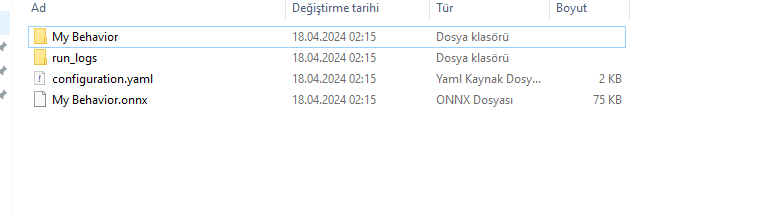
\includegraphics[width=0.9\textwidth]{onnx.PNG}
    \caption{Model Kontrolü} 
    \label{fig:resim17}
    \end{figure}
    

    \subsection{Eğitim Sırasında Hata Ayıklama}
        ML-Agents ile çalışırken, eğitim sırasında ortaya çıkan hataları tanımlamak ve çözmek önemlidir. Bu bölümde, eğitim sırasında sık karşılaşılan hataları ve bunların nasıl çözülebileceğini ele alacağız. Ayrıca, eğitim sürecini izlemek ve modelin performansını değerlendirmek için kullanılabilecek araçlar hakkında bilgi vereceğiz.


\section{Performans Optimizasyonu}
    ML-Agents ile çalışırken, performans optimizasyonu önemli bir konudur, özellikle büyük ölçekli eğitim setleri veya karmaşık ortamlar kullanırken. Bu bölümde, performansı artırmak için kullanılan bazı teknikleri ele alacağız:

    \subsection{Eğitim Süresini ve Maliyeti Azaltma Yöntemleri}
        Eğitim süresini ve maliyetini azaltmak için kullanılabilecek çeşitli teknikler vardır. Bu teknikler arasında veri paralelleştirmesi, model paralelleştirmesi, dağıtık eğitim ve donanım optimizasyonu gibi yöntemler bulunabilir.

    \subsection{İleri Algoritmaların ve Tekniklerin Kullanımı}
        ML-Agents'in yanı sıra, performansı artırmak için kullanılabilecek daha gelişmiş makine öğrenimi algoritmaları ve teknikler de bulunmaktadır. Bu bölümde, daha gelişmiş algoritmaların ve tekniklerin nasıl kullanılabileceğini ve ML-Agents ile entegrasyonunun nasıl sağlanabileceğini ele alacağız.
\clearpage
\bibliographystyle{ieeetr}
\bibliography{referance}

\end{document}
